\chapter{Experiments and Results}\label{ch:ch5}
Given the powerful advances in NLP and music generation tasks, our general goal was to investigate the Transformer model in application to EMP generation. Both language and music are by nature sequential and hierarchical. As such, one would expect the strengths of a Transformer model, created specifically for an NLP task, to have natural extensions into musical tasks (as was shown by the ``Music Transformer'' and OpenAI's generative models).  This project's initial purpose was to determine if a Transformer-based model improves upon \vnet{}, given the same data, features, and evaluation metrics. However, as discussed in chapter \ref{ch:ch6}, answering that question proved to be more complicated than initially anticipated and led our research in a different direction. We present our initial method and experiment results in this chapter. 

We use the complete end-to-end generation system of the \vnetf{}. There are three major reasons for adopting the \vnet{} system. 
\begin{enumerate}
    \item The KAIST dataset is the largest publicly available dataset used in EMP generation.
    \item \vnet{} models are the ``best performing'' in EMP.
    \item The data processing and model architecture code of the \vnetf{} are open-sourced\footnote{\url{https://github.com/jdasam/virtuosoNet}.}.
\end{enumerate}
If we consider \vnet{} to be state-of-the-art in EMP generation, it provides a natural starting place to compare against any further model development. 

\section{Data and Features}
The \vnet{} system uses handcrafted features for both scores and performances, which are outlined in chapter \ref{ch:ch4}. We use the same feature set.

\section{Our Model}
In the \vnet{} system, there is a 1:1 mapping between notes in scores and performances. As mentioned in chapter \ref{ch:ch3}, encoder-decoder \seq{} models with variable-length input/output sequences account for the difference in length by using a generative decoder model which relies on the input encoding. Because our input and output sequences are the same lengths, we saw no need to include a generative decoder. Our model is an encoder-only Transformer model. Sitting on top of the Transformer encoder is a simple FFNN that takes as input the learned representation from the Transformer and maps it to the final output feature set. We use the original absolute positional embedding of~\citet{vaswani2017attention}. The model architecture is shown in Figure \ref{fig:model_architecture}.

\begin{figure}[h]
    \centering
    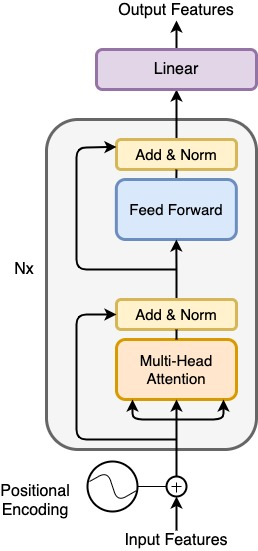
\includegraphics[width=0.3\linewidth]{figs/ch5/model_architecture.jpg}
    \caption{Our model uses the same encoder Transformer architecture as shown by~\citet{vaswani2017attention}. There are $N$ Transformer layers which are composed of multi-head attention and feed-forward mechanisms. There is a simple linear layer at the top of the architecture which creates the final mapping to the output features.}
    \label{fig:model_architecture}
\end{figure}

\section{Experiment Methods}\label{sec:experiments-and-evaluation}
Our initial experiments were designed to answer two questions: 
\begin{enumerate}
    \item Does a Transformer based EMP generation model outperform a similar LSTM based EMP generation model?
    \item Does a Transformer based EMP generation model outperform existing state-of-the-art (\vnet{}) models?
\end{enumerate}
To answer both of these questions, we ran all of our experiments using the existing \vnetf{}. The \vnetf{} defines real-valued features, and the resulting models are regression models. All \vnet{} models use MSE as both the loss function for training and reconstruction error for quantitative evaluation. \vnet{} models are trained using an 8-1-1 train/valid/test data split, and~\citet{jeong2019virtuosonet} present MSE results for several different models. These MSE results are given for each different expressive parameter, including tempo, velocity, deviation (timing), articulation, and pedal. We follow the same method for our quantitative evaluation, using the same data split, loss function, and evaluation metrics. 

Our models were trained for 50 epochs, and the best model parameters were selected according to the lowest validation evaluation score. Our models were implemented in PyTorch using their native Transformer library. We used Neptune AI~\cite{neptune} to manage our experiments and report the metric feedback. Data for all of our experiments, including the model hyperparameters and metrics, can be found online\footnote{\url{http://ui.neptune.ai/richt3211/thesis}.}. 

Our main experimental goal was to find the best model configuration for a Transformer based model. To do so, we ran a reasonably exhaustive hyperparameter search for our Transformer model. To guide our search, we trained our baseline LSTM model and a few \vnet{} models in tandem with our Transformer model. We used the evaluation results from the validation set to gain an intuition about which family of models performed the best. The final test set evaluation happened after all model development was finished. 

\section{Model Evaluation: Quantitative}
We use several different model configurations for the Transformer. Our Transformer baseline has six layers, six attention heads, and a hidden size of 256. We chose this as a base configuration because it closely matches the size of the original Transformer~\cite{vaswani2017attention}, except for the hidden size of the feed-forward layer. We use a smaller hidden size of 256 for our base layer hidden size due to the relatively small dimensionality, 78, of the model's input data% 
\footnote{The original Transformer uses a baseline input dimensionality of 528. In this case, the model inputs are word vectors whose size can be configured dynamically to find the best word representation for a given model. In our case, our input size dimensionality is fixed according to the input features of the \vnetf{}.}.

% my results
%total              %tempo              %vel              %dev              %articul              %pedal        
\readlist*\a{1.08, 0.8387099791654173, 1.3530433499396628, 1.017870266429722, 1.1067559519102133, 1.080384319222477} % 123 
\readlist*\b{0.8634560842141723, 0.5412064723018719, 0.8022146236503704, 0.8804639799541721, 0.8022366483458304, 0.9245564142364828} % 147 
\readlist*\c{0.8714990162701071, 0.5505609703737273, 0.7881732323421042, 0.9611995326543272, 0.8751485813981792, 0.9159152227103448} % 169 
\readlist*\d{0.8608967689267041, 0.5025553895868159, 0.7638317284792879, 0.878050578836977, 0.8178488211257614, 0.929653946913942} % 128 
\readlist*\e{0.83, 0.4671040222800673, 0.7613456284477763, 0.8818908914978052, 0.8233950348666115, 0.8803471737534461} % 133 
\readlist*\f{0.892434075736163, 0.6518531192930515, 0.8248660148758638, 0.8837178772102976, 0.822714017388242, 0.9476605038763138} % 118 
\readlist*\g{0.931571010408277, 0.6190825817829081, 0.96866907527554, 0.8923720742977281, 1.0889969662761827, 0.9540228699651616} % 181 
\readlist*\h{0.8398954164095592, 0.5103522019637757, 0.7708808816209132, 0.9533001596417616, 0.8093733305095236, 0.8849918198915682} % 132 
\readlist*\i{0.9055077961121484, 0.7380731321188851, 0.8207453556958286, 0.9515869074832948, 0.8602034320048559, 0.9414252330302848} % 171 
\readlist*\j{1.005084838962903, 0.8624353822994071, 1.0529326007749042, 0.8987197173990472, 1.1763732810960201, 1.0093531322087683} % 173 
\readlist*\k{0.8352959967855129, 0.6160173766780894, 0.7846170962729531, 0.8910593114013335, 0.7908931125724473, 0.8722384046125028} % 188 
\readlist*\l{0.8463679141699834, 0.5445592460407571, 0.7492400507566016, 0.899280836268869, 0.8597047927381344, 0.8938945523819722} % 134 
\readlist*\m{0.8707426997177073, 0.4897337480780074, 0.7796597156133693, 0.8877784585332059, 0.8655195282458561, 0.9364968512758156} % 190 
\readlist*\n{0.8436574470387758, 0.4748660706616556, 0.8106850048921405, 0.8946506051604983, 0.8585572391965963, 0.8916389604554559} % 135 
\readlist*\o{0.9331073568122104, 0.6931559999619044, 0.9870281539322866, 0.9139575008493828, 1.1235607440091158, 0.9352111728264682} % 125

% virtuosoNet results. Copied from other papers

                        % total      %temp, %vel, %dev, %art, %pedal  
\readlist*\vbl{0.7698181818181818, 0.4, 0.673, 0.773, 0.721, 0.843} 
\readlist*\vs{0.7324545454545454, 0.269, 0.607, 0.753, 0.688, 0.82} 
\readlist*\vm{0.72, 0.22, 0.532, 0.747, 0.754, 0.81}

% lrv for learning rate value. Putting in command so that it doesn't ruin table alignment
\newcommand{\lrv}{\num{3e-5}}

\begin{table}[!htbp]
    \setlength{\tabcolsep}{0.4em}
    \setlength{\extrarowheight}{7pt}
    \sisetup{round-mode=places}
    \begin{center}
    \begin{tabular}{| c c | c c c c c c | S[round-precision=2] S[round-precision=2] S[round-precision=2] S[round-precision=2] S[round-precision=2] S[round-precision=2] |}
        \hline 
        \multicolumn{8}{|c|}{Model Configuration} & \multicolumn{6}{c|}{Results in MSE}\\
        \hline
        \nep & \mn & \nl & \dhid & \drop & \lr & \clip & \nh & Tot & \temp{} & \vel{} & {\dev{}} & \art{} & \ped{} \\ 
        % \nep & \mn & \nl & \dhid & \drop & \lr & \clip & \nh & 1 & 1 & 1 & 1 & 1 & 1 \\ 
        \hline 
123 & \textbf{LSTM}   & 3  & 256  & 0.1 & 0.1     & 0.5 &    & \textbf{      \a[1]} & \a[2] & \a[3] & \a[4] & \a[5] & \a[6] \\ 
\hline
147 & T-BL   & 6  & 256  & 0.1 & 3e-5    & 0.5 & 6  & \b[1] & \b[2] & \b[3] & \b[4] & \b[5] & \b[6] \\
169 &        &    & 128  &     &         &     &    & \c[1] & \c[2] & \c[3] & \c[4] & \c[5] & \c[6] \\
128 &        &    & 528  &     &         &     &    & \d[1] & \d[2] & \d[3] & \d[4] & \d[5] & \d[6] \\
\textbf{133} & \textbf{T-Best} &  & 1024 & & &   &    & \textbf{      \e[1]} & \e[2] & \e[3] & \e[4] & \e[5] & \e[6] \\
118 &        & 12 &      &     &         &     &    & \f[1] & \f[2] & \f[3] & \f[4] & \f[5] & \f[6] \\
181 &        & 24 &      &     &         &     &    & \g[1] & \g[2] & \g[3] & \g[4] & \g[5] & \g[6] \\
132 &        &    &      &     &         &     & 13 & \h[1] & \h[2] & \h[3] & \h[4] & \h[5] & \h[6] \\
171 &        &    &      & 0.2 &         &     &    & \i[1] & \i[2] & \i[3] & \i[4] & \i[5] & \i[6] \\
173 &        &    &      &     & 0.01    &     &    & \j[1] & \j[2] & \j[3] & \j[4] & \j[5] & \j[6] \\
188 &        &    &      &     &         &     & 26 & \k[1] & \k[2] & \k[3] & \k[4] & \k[5] & \k[6] \\
134 &        & 12 & 528  &     &         &     &    & \l[1] & \l[2] & \l[3] & \l[4] & \l[5] & \l[6] \\
190 &        & 12 &      &     &         &     & 13 & \m[1] & \m[2] & \m[3] & \m[4] & \m[5] & \m[6] \\
135 &        & 12 & 528  &     &         &     & 13 & \n[1] & \n[2] & \n[3] & \n[4] & \n[5] & \n[6] \\
125 & T-Worst& 24 & 528  &     &         &     &    & \o[1] & \o[2] & \o[3] & \o[4] & \o[5] & \o[6] \\
\hline
& HAN-BL &  - &  -   &  -  &    -    &  -  &  - & \vbl[1] & \vbl[2] & \vbl[3] & \vbl[4] & \vbl[5] & \vbl[6] \\
& HAN-S  &  - &  -   &  -  &    -    &  -  &  - & \vs[1]  & \vs[2]  & \vs[3]  & \vs[4]  & \vs[5]  & \vs[6] \\
& \textbf{HAN-M}  &  - &  -   &  -  &    -    &  -  &  - & \textbf{     \vm[1]}  & \vm[2]  & \vm[3]  & \vm[4]  & \vm[5]  & \vm[6] \\
        \hline
    \end{tabular}
    \caption{A comparison of 3 different families of EMP generation models: \vnet{} models, Transformer models, and our LSTM baseline models. \nep{} is the ID of the Neptune experiment, \nl{} is the number of layers, \dhid{} is the dimension of the hidden layers, \drop{} is the dropout, \lr{} is the learning rate, \clip{} is the gradient clip, and \nh{} is the number of attention heads. Empty spaces for the Transformer configuration values imply the baseline value (for example, the number of layers for model 169 is 6). The right side of the table presents the MSE results for all models along the five different expressive parameters used in the \vnetf{}, as well as the total MSE which is an aggregation of all the individual expressive features. The entries for the HAN models come from \vnet{} and are given by~\citet{jeong2019virtuosonet}. }
    \label{tab:quantitative}
    \end{center}
\end{table}

Table \ref{tab:quantitative} contains the full results of the final evaluation and includes MSE results for all of the different Transformer models, our baseline LSTM model, and the best performing \vnet{}.

As shown in Figure \ref{fig:experiment_results}, the first major implication of the results is that the Transformer model easily outperforms the baseline LSTM but does not outperform the \vnet{} models. The best performing Transformer model uses all of the same baseline Transformer parameters, except for a major increase in the hidden layer's dimensionality (this is found in model \tm{133}, we use the notation $T_{N_{i}}$ to refer to the Neptune ID of a Transformer model.). Other models that perform well include those which only increase the number of attention heads (\tm{132} and \tm{26}) and those with an increase across several different parameters (\tm{135}). It appears that increasing the number of layers degrades performance (\tm{118}, \tm{181}, \tm{125}), and so does increasing the dropout and learning rates (\tm{171}, \tm{173}). 

\begin{figure}[!b]
    \centering
    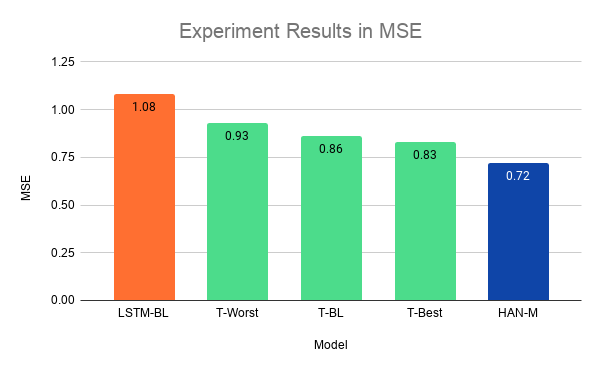
\includegraphics[width=0.8\linewidth]{figs/ch5/experiment_results.png}
    \caption{Results for the three different model families, LSTM baseline, Transformer, and \vnet{}, are shown in different colors. There is a substantial difference in results for each model family, with the LSTM baseline performing the worst, \vnet{} performing the best, and the Transformers sitting in between.}
    \label{fig:experiment_results}
\end{figure}

Although we see improvements by increasing the hidden dimension and number of attention heads, the performance improvements are not notable. There is only a difference of 0.03 in MSE between the best performing Transformer model and the Transformer baseline. In contrast, there is a difference of 0.11 between the best Transformer model and the best HAN model. An initial interpretation of these results would indicate that a Transformer model can not even match the existing state of the art in EMP generation (let alone beat it). As we discuss in the following section, this interpretation of results is not necessarily valid. 